\documentclass[]{jarticle}          % 一段組
%\documentclass[twocolumn]{jarticle} % 二段組

\textwidth 180mm
\textheight 255mm
\oddsidemargin -12mm
\topmargin -15mm
\columnsep 10mm

%\vspace{0.5cm} % 一段組の場合はコメントアウトした方が体裁がよいx
%] % 一段組の場合はコメントアウトする

\usepackage{styles/labheadings}
\usepackage[dvipdfmx]{graphicx,color}
\usepackage{amsmath,amssymb}
\usepackage{url}
% 追加
\usepackage[hang,small,bf]{caption}
\usepackage[subrefformat=parens]{subcaption}
\usepackage{float}
\captionsetup{compatibility=false}

\input{numerical_definition.tex}
% report.texと同じディレクトリにnumerical_definition.texを入れておけば上の書き方でもいいはずです

\usepackage[
  dvipdfm,
  bookmarks=true,
  bookmarksnumbered=true,
  colorlinks=true]{hyperref}
\AtBeginDvi{\special{pdf:tounicode EUC-UCS2}}

\pagestyle{labheadings}
\headerleft{2次元フロアマップからのシーンの3次元モデルの作成}   % ヘッダの左側のタイトル
\headerright{2024年1月29日}  % ヘッダの右側のタイトル

\begin{document}

%\twocolumn % 一段組の場合はコメントアウトする

\vspace*{2ex}
\begin{center}
 {\Large \bf テクスチャと入力画像の対応付けの自動化}\\ % タイトル
 \vspace*{5mm}
 {\large M2 田川幸汰}% 発表者名
\end{center}

%\vspace{0.5cm} % 一段組の場合はコメントアウトした方が体裁がよいx
%] % 一段組の場合はコメントアウトする

%新しく作成したコマンド
% \newcommand{\reffig}[1]{\hyperref[#1]{図\ref{#1}}}
% \newcommand{\refeq}[1]{\hyperref[#1]{式(\ref{#1})}}
% \newcommand{\reftab}[1]{\hyperref[#1]{表\ref{#1}}}
% \newcommand{\refsec}[1]{\hyperref[#1]{\ref{#1}章}}
% \newcommand{\refsubsec}[1]{\hyperref[#1]{\ref{#1}節}}

% 数式
%\begin{equation}
%  数式記述  
%  \label{ラベル名}
%\end{equation}

% 図
% \begin{figure}[!ht]
%   \begin{center}
%     \includegraphics[scale=0.5]{figures/画像ファイル名}
%     \caption{キャプション名}
%     \label{ラベル名}
%   \end{center}
% \end{figure}

% リスト
% \begin{enumerate or itemize}
%   \item 
% \end{enumerate or itemize}

\section{概要}
前回までの報告では、全方位画像から3次元モデルのテクスチャを割り当て、自己位置推定を行った。
従来のテクスチャを用いた自己位置推定手法では、特徴点の選択や対応付けが手動で行われており、実用的な運用には限界があった。
本報告では、自己位置推定における特徴点の選択や対応付けを自動化し、より実用的な手法を提案する。
入力画像1枚に対して複数のテクスチャ画像が存在するが、全てのテクスチャに対して特徴点マッチングを行うと実行時間が大幅に増加し、リアルタイムでの処理は困難である。
そのため、本研究ではcoarse to fineな手法を採用する。
具体的には、まず入力画像とテクスチャ画像の全体的な特徴を捉える大域特徴量を用いた類似画像検索を行い、候補となる画像の数を大幅に削減する。
その後、選択された類似画像に対して局所特徴量を用いた詳細な特徴点マッチングを実施することで、精度と処理時間のバランスを取る。

\section{大域特徴量による類似画像検索}
あらかじめ全てのテクスチャ画像に対して特徴量を抽出し、データベースを作成しておく。
入力画像が与えられた際には、その特徴量を算出し、データベース内のテクスチャ画像の特徴量と比較することで、最も類似した特徴を持つテクスチャ画像を類似画像として求める。
入力画像と検索対象のテクスチャ画像は形状変化が大きいため、それらに対してロバストな特徴を用いる。
本研究では大域特徴として深層学習による大域特徴量抽出手法であるResNetによって得られた特徴を用いて類似画像検索を行い、特性を評価した。

\subsection{実験結果の比較}
ResNetを用いた場合の類似画像検索の結果を図\ref{one}に示す。なお上の画像から奥行き方向に左向きに90°、60°、30°回転させた画像を入力画像としている。
\begin{figure}[H]
  \begin{center}
    \begin{tabular}{c}
      \includegraphics[width=0.7\textwidth]{figures/RasNet270.png}\\
      \includegraphics[width=0.7\textwidth]{figures/RasNet300.png}\\
      \includegraphics[width=0.7\textwidth]{figures/RasNet330.png}\\
    \end{tabular}
  \end{center}
  \caption{類似画像検索}
  \label{one}
\end{figure}
ResNetを用いた類似画像検索の結果から、入力画像とテクスチャ画像の相対的な向きによって、検索結果や特徴点マッチングの精度に違いが生じることが確認された。
入力画像がテクスチャ画像に対して正面を向いている場合、大域特徴量を用いた類似画像検索は安定して機能し、適切なテクスチャ画像を高精度に選択できる。
しかし、入力画像がテクスチャ画像の正面を向いている場合、画像内の線特徴が乏しくなり、線特徴を用いたマッチングの精度が低下する。
一方、入力画像がテクスチャ画像に対して斜めを向いている場合、視点変化の影響で画像の形状が大きく変化する。その結果、大域特徴量のみを用いた類似画像検索の精度が低下する傾向が確認された。
しかし、斜めを向いた画像では、奥行き方向の線特徴が顕著に現れるため、それらを活用することで特徴点マッチングの精度向上が期待できる。
点特徴と線特徴を適切に組み合わせることで、それぞれの弱点を補完し、より高精度なマッチングの実現が可能であると考えられる。

\section{局所特徴量による特徴点マッチング}
入力画像とテクスチャ画像のより精密な対応付けを行うため、局所特徴量を用いた特徴点マッチングを実施する。
特徴点マッチングの手順として、まず各画像から特徴点を検出し、特徴記述子を作成する。
その後、FLANN(Fast Library for Approximate Nearest Neighbors)を用いて、記述子同士の対応を求める。
FLANNは、高速な近似最近傍探索を行うライブラリであり、大規模な特徴点データに対して効率的に類似する点を検索できる。
マッチング後、RANSAC(Random Sample Consensus)アルゴリズムを適用し、外れ値を除去する。
RANSACは、ランダムにサンプルを選択してモデルを作成し、外れ値を排除する手法であり、誤対応を減らし精度の高いマッチングを実現する。
最終的に、良いマッチと判断された特徴点のペアの個数が最も多いテクスチャ画像を自己位置推定に用いる。
本研究ではSIFT、AKAZE、ORBの特徴点検出器を用いて特徴点マッチングを行い、特性を比較・評価した。

\subsection{実験結果の比較}
それぞれの特徴を用いた場合の特徴点マッチングの結果を図\ref{two}に示す。
なお、奥行き方向に左向きに30°回転させた画像を入力画像として、上からSIFT、AKAZE、ORBの特徴点検出器を使用している。
また、マッチングの結果は上位10点を表示している。
\begin{figure}[H]
  \begin{center}
    \begin{tabular}{c}
      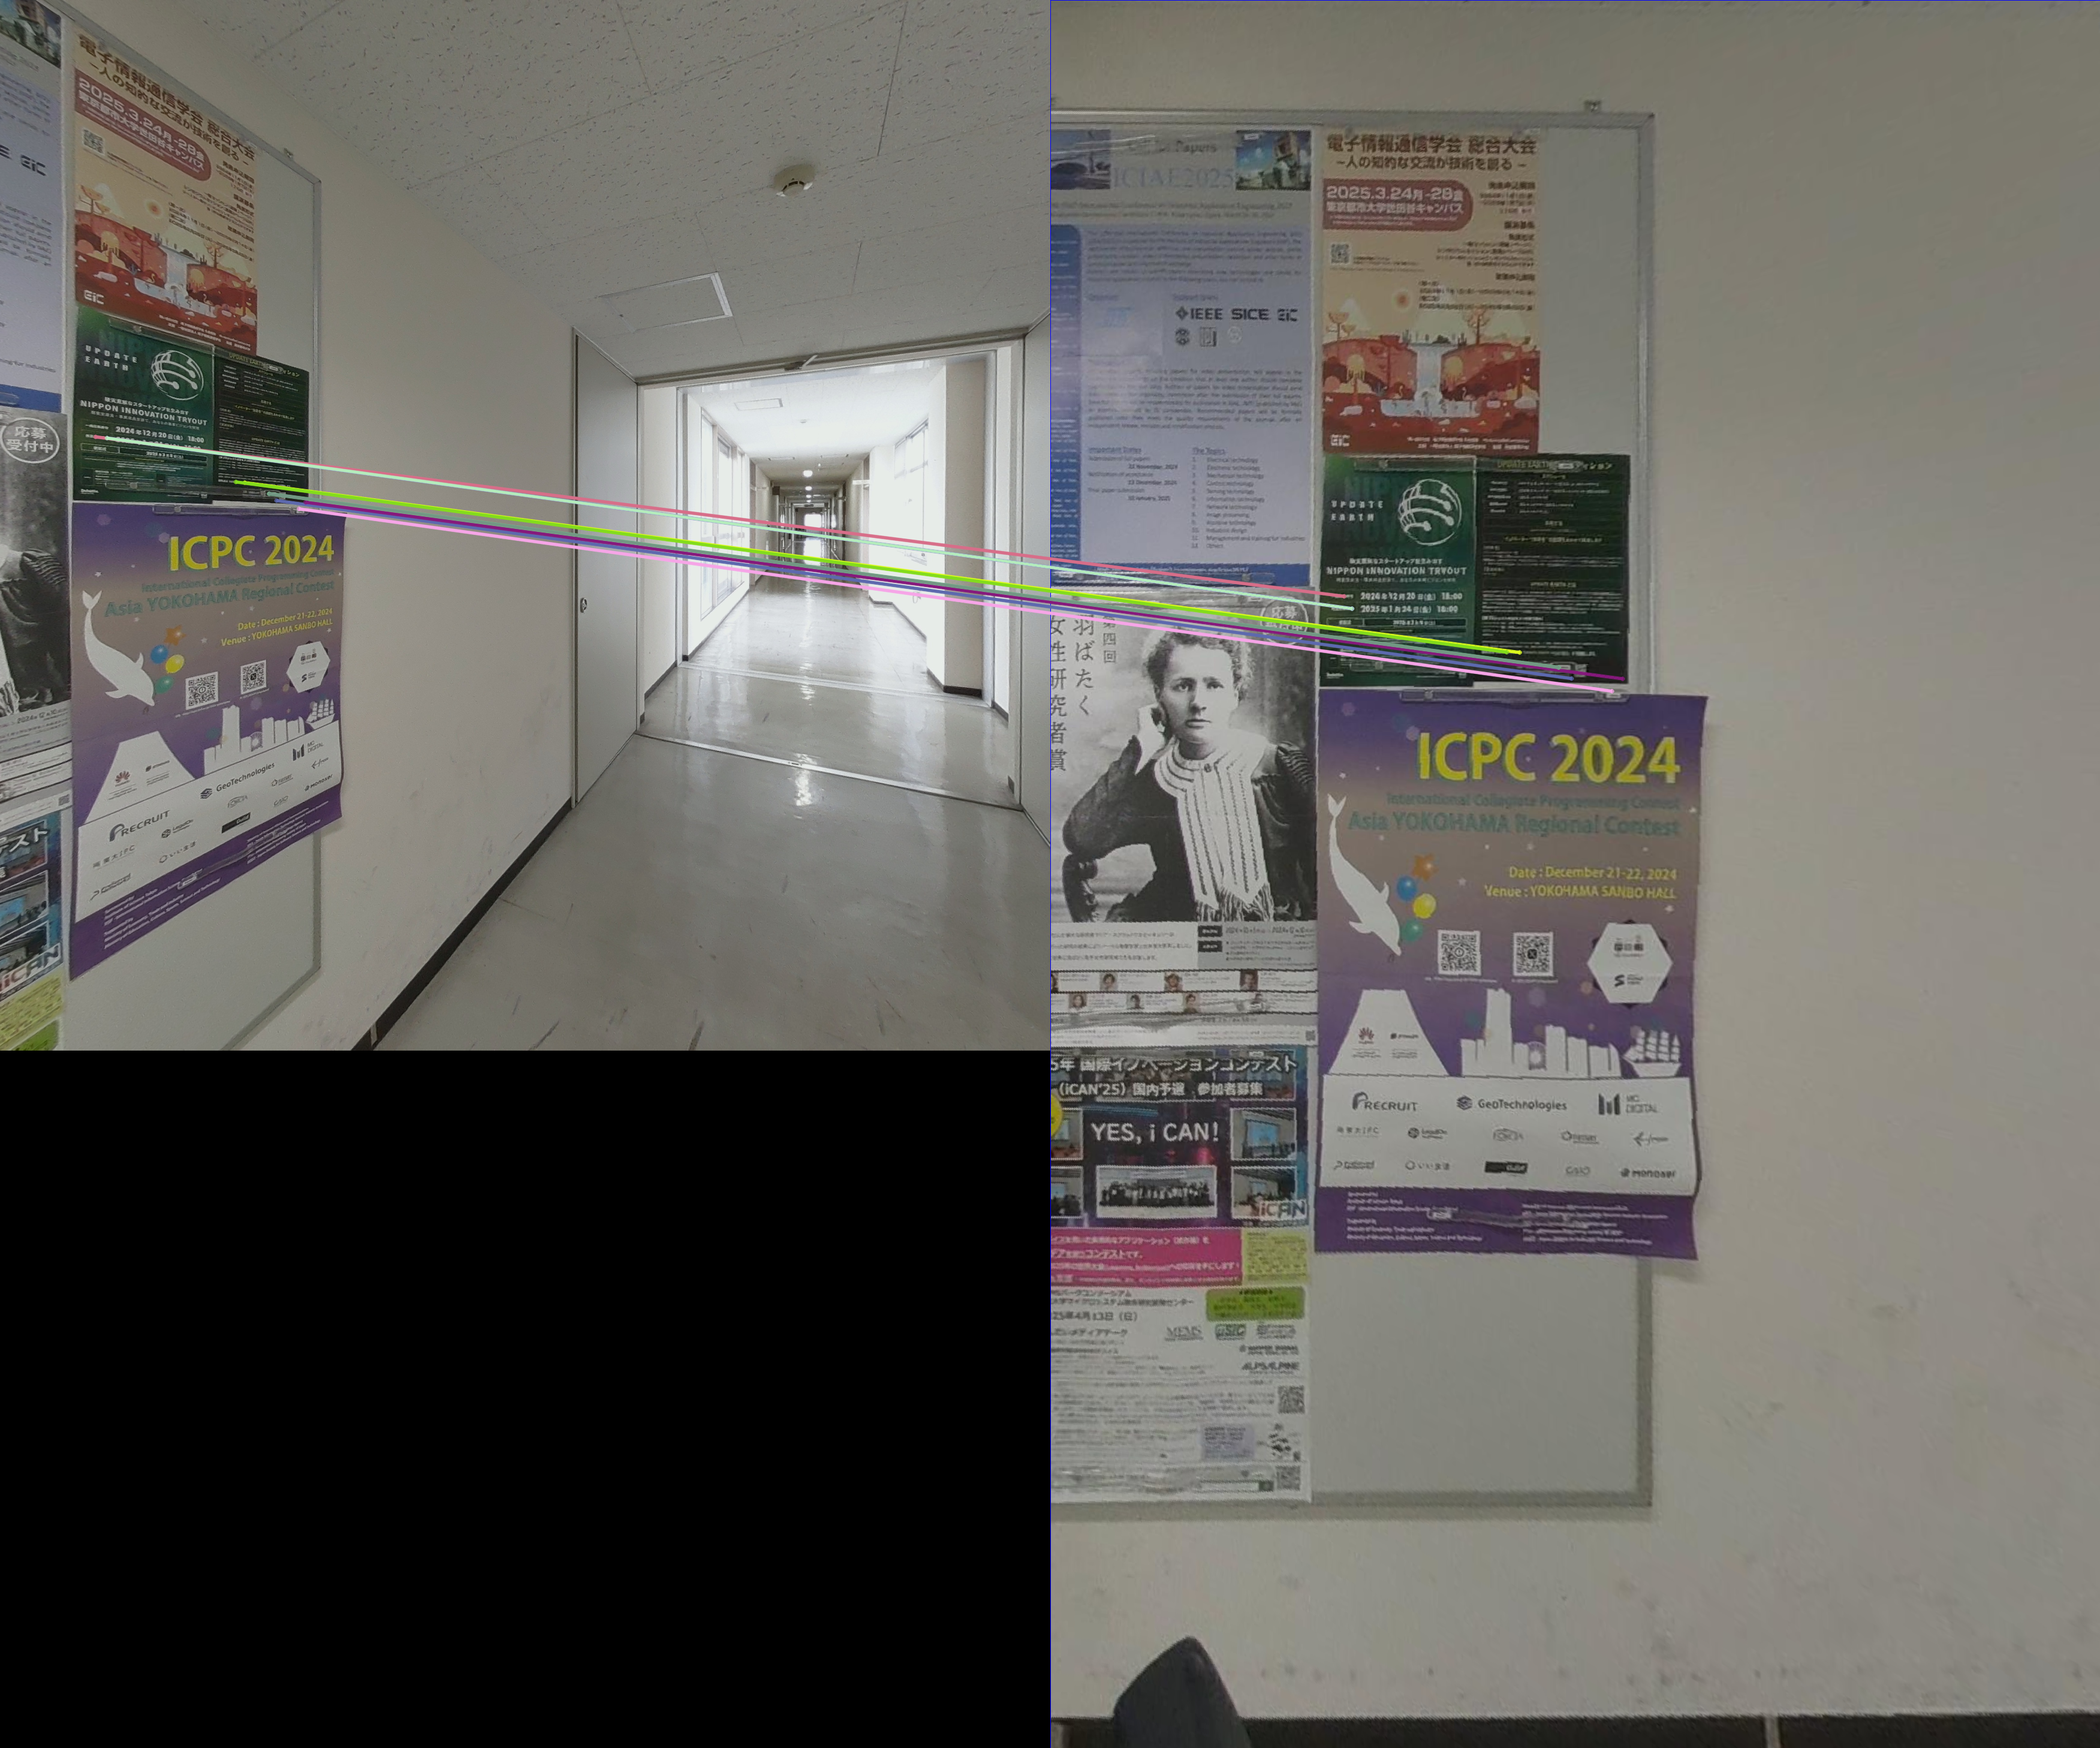
\includegraphics[width=0.5\textwidth]{figures/SIFT_result.png}\\
      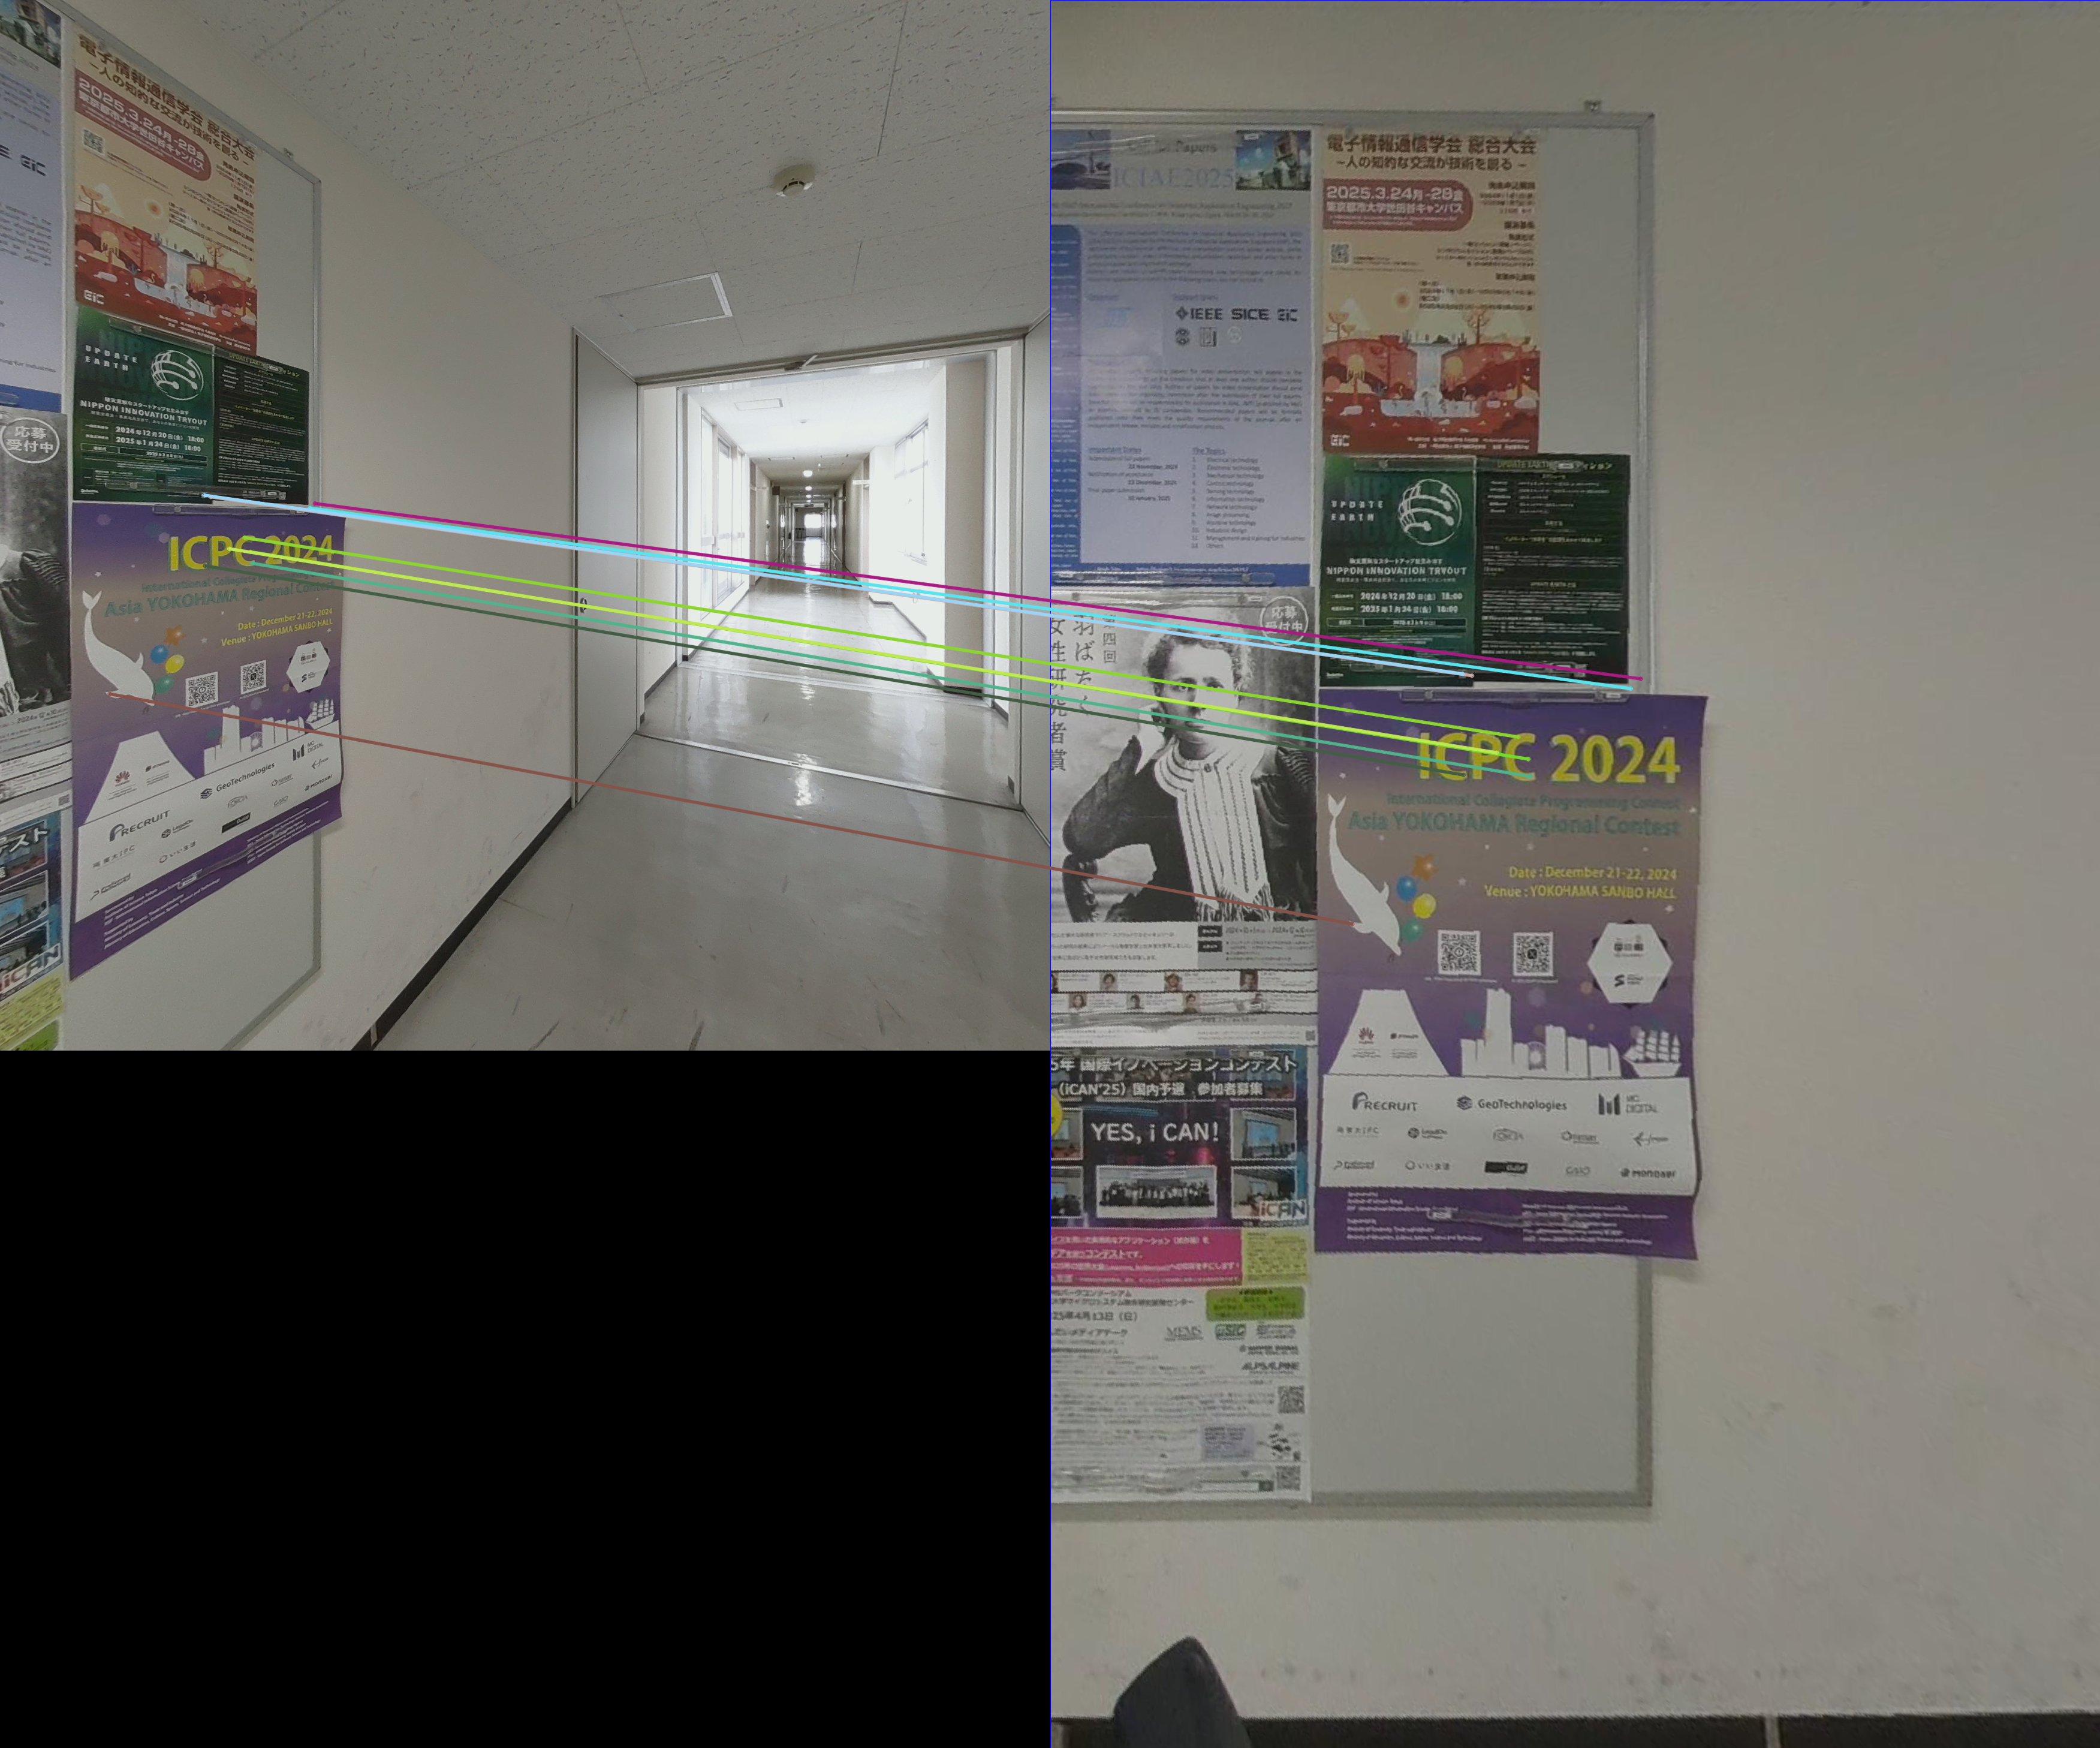
\includegraphics[width=0.5\textwidth]{figures/AKAZE_result.png}\\
      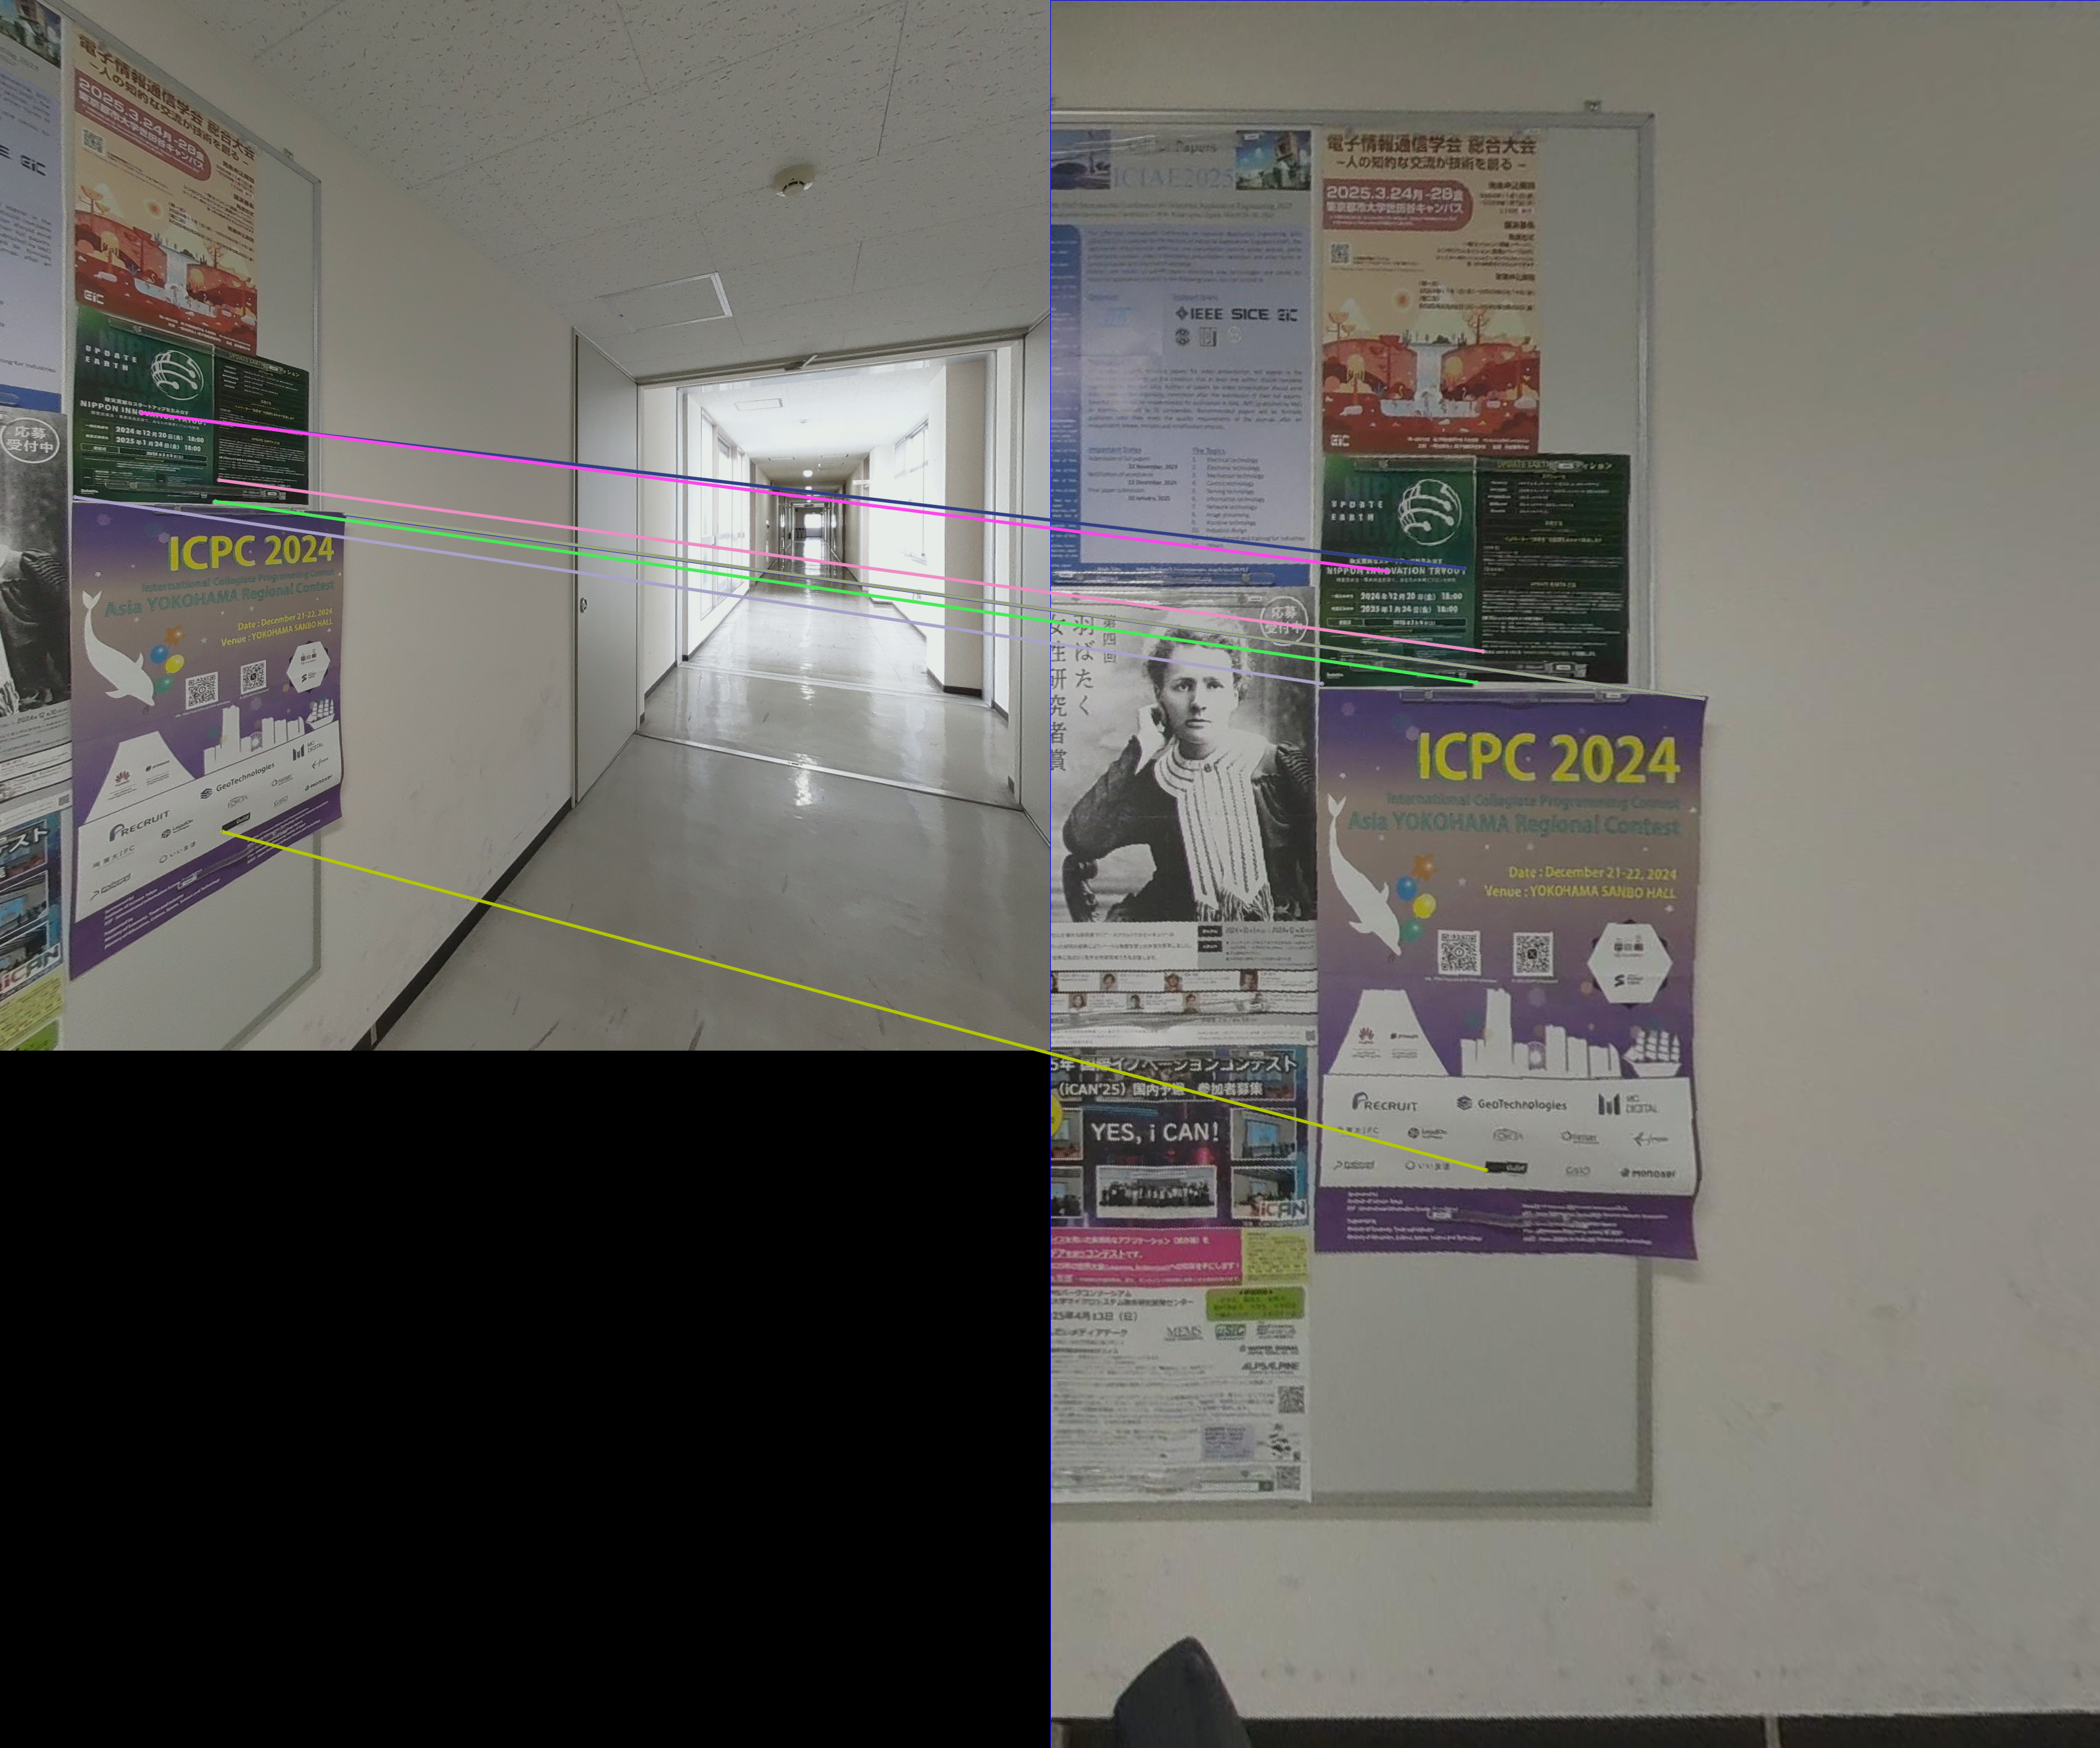
\includegraphics[width=0.5\textwidth]{figures/ORB_result.png}\\
    \end{tabular}
  \end{center}
  \caption{特徴点マッチング}
  \label{two}
\end{figure}

いずれの特徴点検出器を使用しても、正しく特徴点マッチングが行われていることが確認できた。
特に、局所特徴量に基づく特徴点マッチングは、大域特徴量を用いる場合に比べて、視点変化による画像の形状変化に対して非常に剛健であることがわかる。
これは、視点変化が大きくても、局所的な特徴点が安定してマッチングできるため、特に回転やスケール変化がある場合でも有効であることを示唆している。
また、各検出器を用いた場合の特徴点マッチ数と実行時間を表\ref{three}に示す。
\begin{figure}[H]
  \begin{center}
    \begin{tabular}{lcc}
    & 特徴点マッチ数 & 実行時間(s) \\
    SIFT & 101 & 4.03238 \\
    AKAZE & 653 & 2.64763 \\
    ORB & 45 & 0.39160
    \end{tabular}
  \end{center}
  \caption{各検出器の比較}
  \label{three}
\end{figure}
AKAZEは特徴点のマッチ数において優れており、ORBは実行速度において非常に優れていることがわかる。ただし、ORBは場合によって十分な特徴点を検出できないことがあり、
特に複雑な視点変化を伴う画像においてその限界が現れることが確認された。
そのため、本研究では、特徴点マッチングの精度と安定性を考慮し、AKAZEを使用する。

\section{ResNetとAKAZEを用いたcoarse to fineな手法による類似画像検索}
ResNetとAKAZEを用いた場合の類似画像検索結果について図\ref{three}に示す。
なお、類似度$Sim$は以下の式で表す。
\begin{equation}
  Sim = ResNet_{score}\times{0.5}+(AKAZE_{matchcount}/100)\times{0.5}
\end{equation}
\begin{figure}[H]
  \begin{center}
    \begin{tabular}{c}
      \includegraphics[width=0.7\textwidth]{figures/RasNet_AKAZE330.png}\\
    \end{tabular}
  \end{center}
  \caption{ResNetとAKAZE}
  \label{four}
\end{figure}
ResNet単体では、入力画像がテクスチャ画像に対して斜めを向いている場合、特徴量抽出の精度が低下し、類似画像検索の精度にも影響を与える。
しかし、AKAZEのスコアを組み合わせることで、視点変化や回転に強い局所特徴を利用でき、より正確に類似画像を検索することができた。
この結果、AKAZEとResNetを組み合わせることで、精度の向上だけでなく、検索速度の面でも優れたパフォーマンスを実現した。
具体的には、AKAZEを全ての画像に適用する場合と比較しても、ResNetとAKAZEの組み合わせによって、より効率的に処理を行うことができ、実行時間を短縮することができた。
\section{今後の計画}
今後の研究では、まずResNetとAKAZEを組み合わせた特徴点対応を用いて自己位置推定を実施し、
全体の実行時間と自己位置推定の精度を詳細に評価する。
具体的には、ResNetを使用して類似画像検索を行い、AKAZEによる特徴点マッチングを基に自己位置推定を実施する。
さらに、現行の手法の改善を目指して、効率化や精度向上を図るための新たな手法の検討を進めます。
例えば、線特徴の活用を視野に入れ、線分やエッジ情報を取り入れることで、テクスチャだけでなく環境の構造的特徴をより有効に捉えることができる可能性がある
\end{document}
